%\chapter{Density-dependent Flow -- HC or THC}

\section{Theory}
\subsection{Governing Equations}\label{SS:GoverningEquation}

The governing equations used for variable density flow consist of
three fundamental conservation equations: (i) continuity equation of
flow, (ii) momentum equation, and (iii) contaminant transport
equation. In addition, these three equations are linked to the
equations of the bulk fluid density and the hydrodynamic dispersion
equations.

\subsubsection{Equation of the Bulk Fluid Density}\label{SS:BulkFluidDensity}
The linearized equation of the bulk fluid density under an
isothermal state was formulated in terms of hydraulic head as,

\begin{equation}\label{bulkfluiddensity}
\rho  = \rho _0 \left( {1 + \lambda _h \left( {h - h_0 } \right) +
\lambda _c C} \right)
\end{equation}

where $h$ is the hydraulic head, $\lambda$ is the reference
hydraulic head, $\rho$ is the density of fluid, $\rho _0$ is the
reference density of the fluid, $\lambda _h$ represents the
coefficient of compressibility of the fluid associated with the
change of the hydraulic head at constant mass fraction of the
solute, $\lambda _C$ is the coefficient of expansivity resulting
from the change of the mass concentration of the solute at constant
hydraulic head, and $C$ is the relative concentration.

The relationship between density and concentration can also be
approximated using other representations such as an exponential
function as given by Kolditz et al. [1998]. The equations describing
the relationship between density and other relevant parameters are
formulated based on experiments and are approximate relationships.

Another equation for describing the relationship between density and
concentration (or mass fraction) is provided by Herbert at al.
[1988] and used by Oldenburg and Pruess [1995]. This equation was
derived from the assumption that when two liquids are well mixed,
the masses or the volumes of respective components are additive. In
this study, among these equations which describe the relationship
between density and concentration, the linear equation obtained from
the experiments is chosen to describe the relation between the bulk
fluid density and concentration.

\subsubsection{Continuity equation of flow}\label{SS:ContinuityFlowEquation}

The macroscopic mass balance equation of the fluid averaged over a
representative elementary volume (REV) in a porous medium is

\begin{equation}\label{continuityflow}
\frac{{\partial \left( {S\phi \rho } \right)}}{{\partial t}} +
\nabla  \cdot \left( {\phi \rho \vec v} \right) = \rho Q_\rho
\end{equation}

where $S$ is the saturation ratio, $\phi$ is the porosity, $t$ is
the time, $\vec v$ is the fluid velocity vector, and $\rho Q_\rho$
is the source term of the fluid mass in an aquifer. Based on
Equation \ref{continuityflow}, the flow equation for a variably
saturated porous medium can be written in terms of hydraulic head
and mass concentration,

\begin{equation}\label{continuityflowexpanded}
\phi \frac{{\partial S}}{{\partial t}} + SS_0^h \frac{{\partial
h}}{{\partial t}} + S\phi \lambda _C \frac{{\partial C}}{{\partial
t}} + \nabla  \cdot \vec q + \lambda _c \vec q \cdot \nabla C =
Q_\rho
\end{equation}

where $S_0^h$ is the specific storativity of a porous medium with
respect to hydraulic head change and $\vec q$ is the Darcy velocity
vector. The head-based flow equation, Equation
\ref{continuityflowexpanded}, has the advantage over pressure-based
flow equations because numerically large static pressures may
dominate the dynamic pressure differences that cause motion. The
resulting pressure-based numerical scheme may therefore operate at
less than optimum numerical efficiency. A more efficient way is to
write the flow equation in terms of a quantity that can be directly
related to the driving forces. Such a quantity is the equivalent
freshwater hydraulic head, defined as $h = \frac{p}{{\rho _0 g}} +
z$ [Frind, 1982].

\subsubsection[Momentum Equation of Flow and Dispersive Flux]{Momentum equation of flow (the Darcy Equation) and dispersive flux}\label{SS:MomentumAndDispersion}

The momentum balance equation for variable-density fluid flow in a
porous medium in terms of hydraulic head can be given as

\begin{equation}\label{DarcyEquation}
\vec q = \phi \vec v =  - \frac{{\hat k\rho _0 \vec g}}{\mu }\left(
{\nabla h + \left( {\frac{{\rho  - \rho _0 }}{{\rho _0 }}}
\right)\vec e} \right)
\end{equation}

where $\hat k$ is the tensor of permeability of a porous medium and
$\vec e$ is the unit vector in the gravitational direction. The
dispersion tensor can be written as Bear [1979]

\begin{equation}\label{DispersiveFlux}
\mathord{\buildrel{\lower3pt\hbox{$\scriptscriptstyle\frown$}} \over
D}  = \gamma D_m \hat \delta  + \alpha _T \left| v \right|\hat
\delta  + \left( {\alpha _L  - \alpha _T } \right)\frac{{\vec v_i
\vec v_j }}{{\left| v \right|}}
\end{equation}

where $\gamma$ is the tortuosity, $D_m$ is the coefficient of
molecular diffusion, $\hat \delta$ is the Kronecker-delta (unit
tensor), $\alpha _T$ is the transverse dispersivity, $v$ is the
characteristic value of macroscopic velocity, $\alpha _L$ is the
longitudinal dispersivity, and $i$ and $j$ are the velocities in and
directions respectively.

\subsubsection{Solute transport equation}\label{SS:ContaminantTransport}

The solute transport with a source is governed by the following
advection-dispersion equation

\begin{equation}\label{ContaminantTransportEquation}
\frac{{\partial \left( {\phi C} \right)}}{{\partial t}} + \nabla
\cdot \left( {\phi \vec vC} \right) - \nabla  \cdot \left( {\phi
\hat D \cdot \nabla C} \right) = Q_C
\end{equation}

where $Q_C$ is the source term of the solute in terms of mass
concentration. Ignoring the expansivity resulting from the change of
mass concentration $\lambda _C$, Equation
\ref{ContaminantTransportEquation} can be written as follows

\begin{equation}\label{ContaminantTransportExpandedEquation}
\phi \frac{{\partial C}}{{\partial t}} + \left( {1 - \phi }
\right)\lambda _h C\frac{{\partial h}}{{\partial t}} + \phi \vec v
\cdot \nabla C - \nabla  \cdot \left( {\phi \hat D \cdot \nabla C}
\right) + CQ_\rho   = Q_C
\end{equation}

Kolditz et al. [1998] defined approximation level of density
variations in the mass equations when Equation \ref{continuityflow}
and \ref{ContaminantTransportEquation} are expanded.

%--------------------------
%\section{The Elder Problem}
%
%\subsection{Definition}
%
%\begin{description}
%  \item[Purpose:] To verify density-dependent flow such as free
%  convection, seawater intrusion, and possibly enhanced gas recovery
%  with CO2.
%
%\item[Model description:] The elder problem is a good example of
%free convection phenomena, where the fluid flow is driven purely by
%the density differences of the fluids. Figure \ref{ElderProblemBC}
%illustrates the boundary conditions of the Elder problem. Table
%\ref{TableElder} presents the specific parameters for the Elder
%problem used in this application.
%\end{description}
%
%\begin{figure}[h]
%\centering
%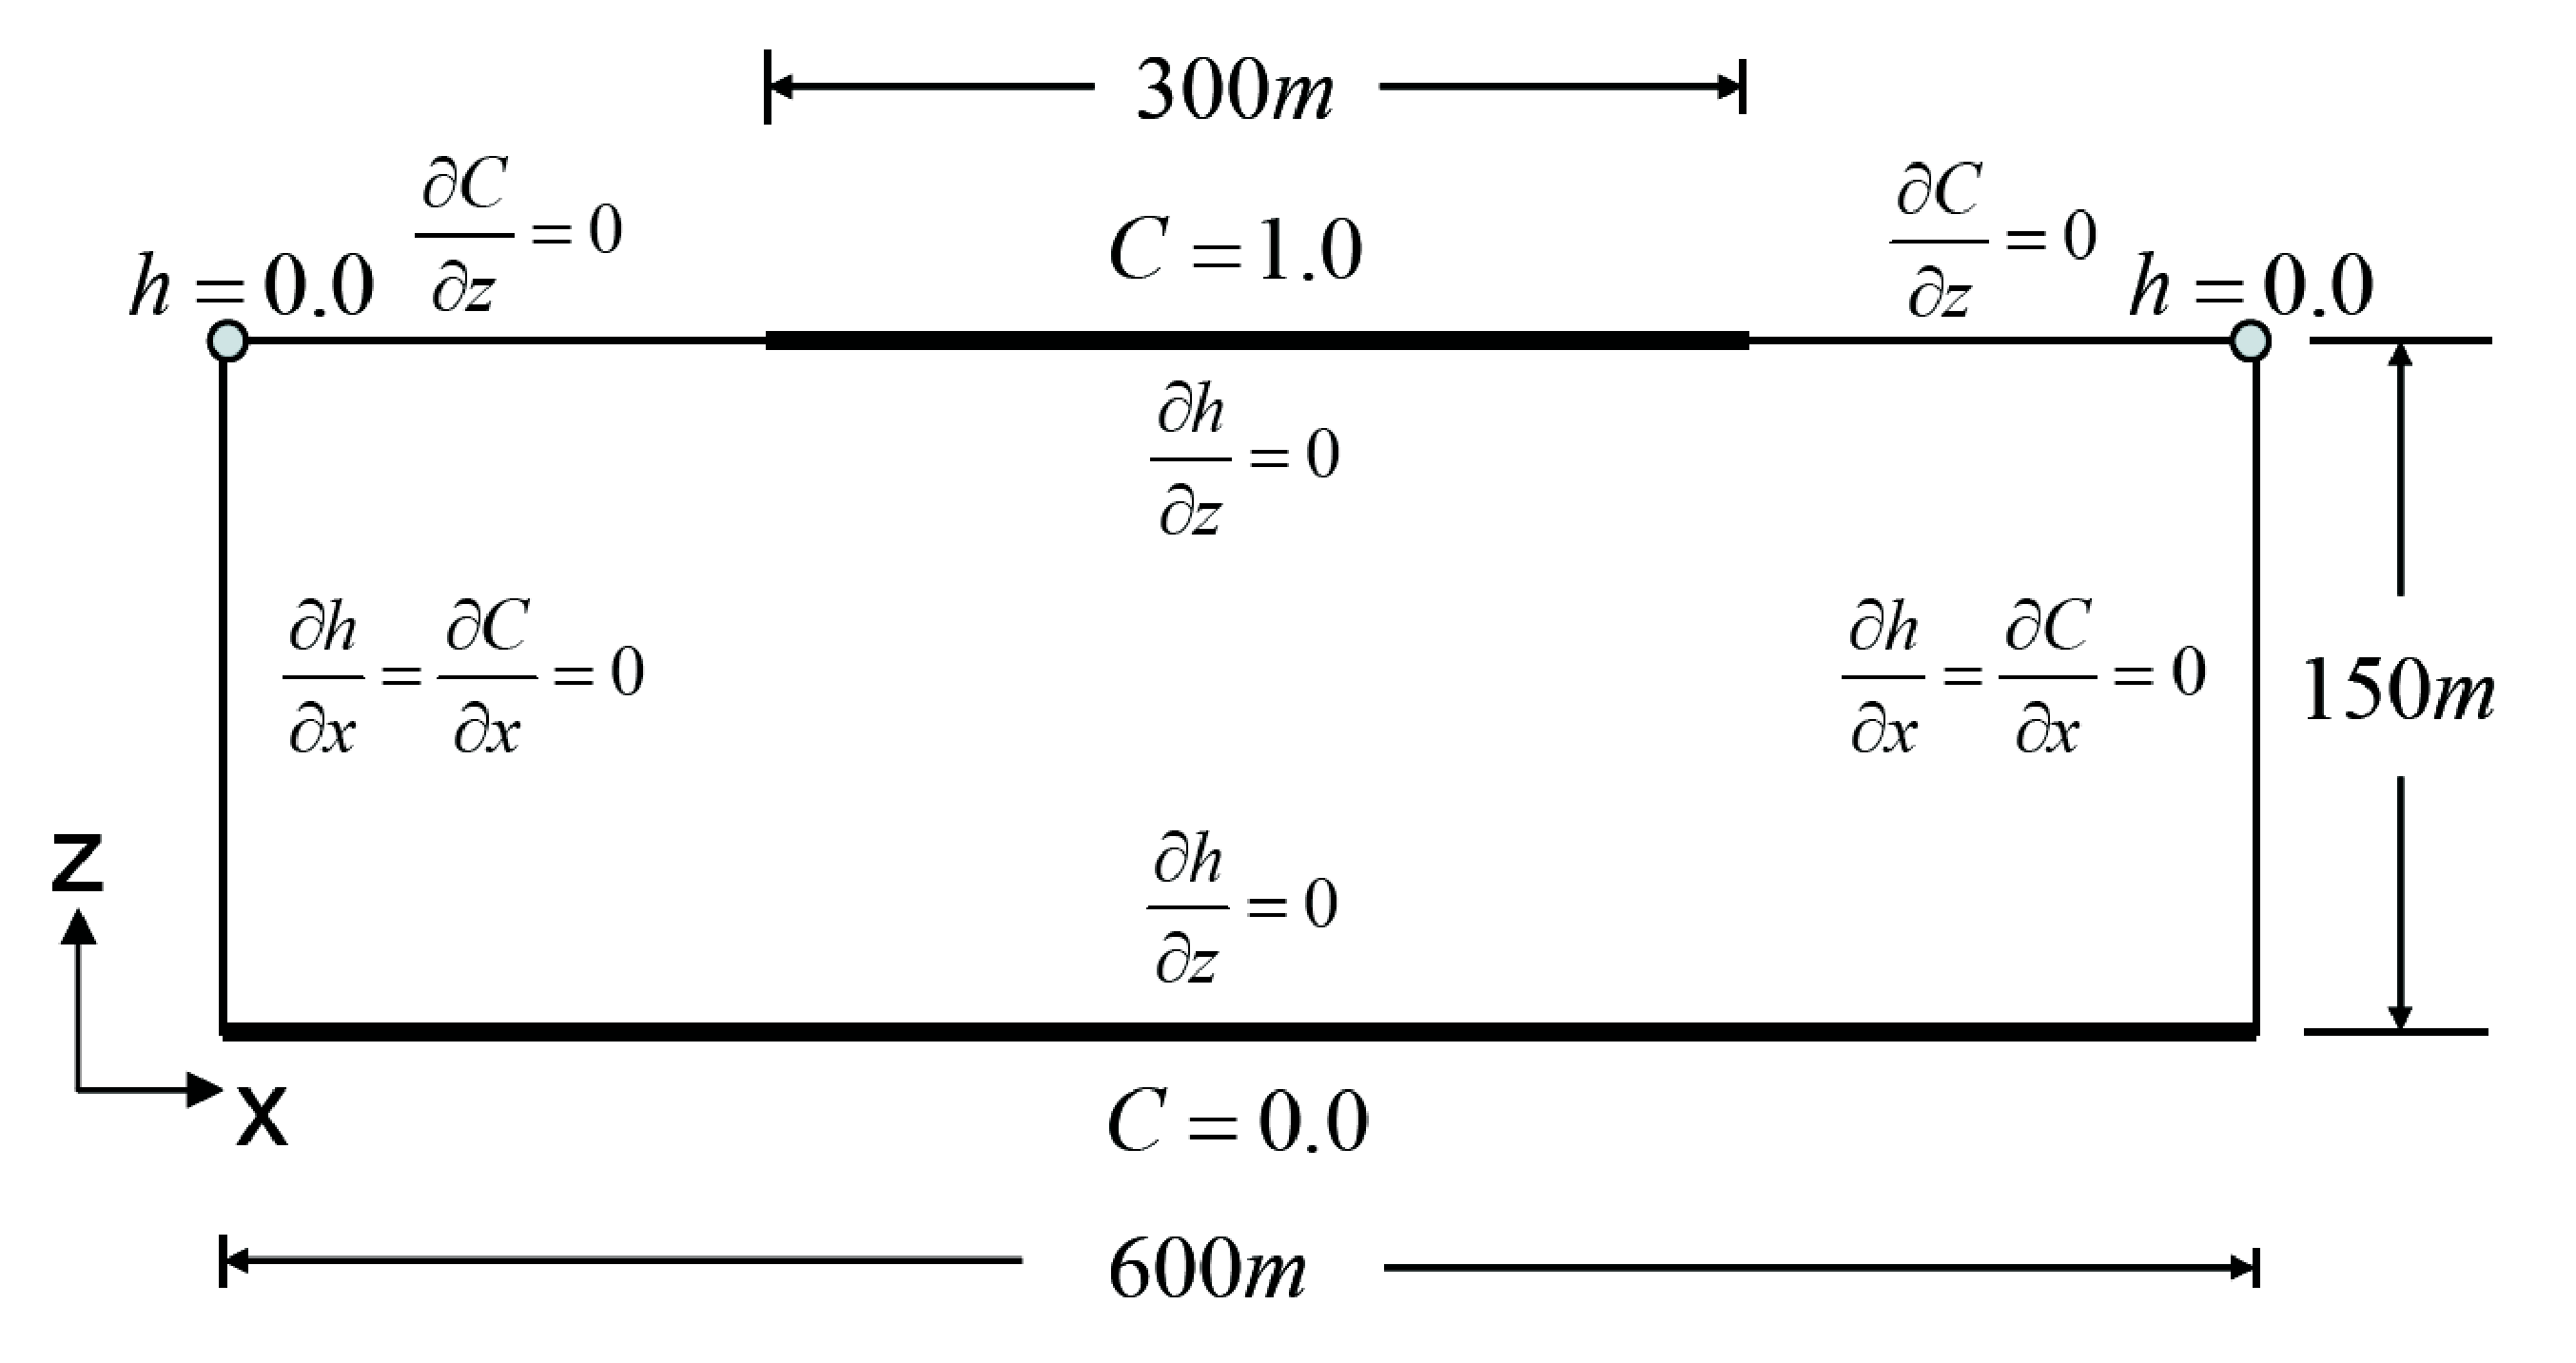
\includegraphics[scale=0.25]{PART_III/DDF/figures/elder_bc.eps}
%\caption{Boundary conditions of the Elder problem}
%\label{ElderProblemBC}
%\end{figure}
%
%\begin{table}[H]
%\begin{center}
%\begin{tabular}{llll}
%\hline \hline
%Symbol & Quantity   &  Value  & Unit\\
%\hline \hline
% $D _m$ & Molecular diffusion coefficient & 3.565e-6  &  $m^2 s^{ - 1}$ \\
% $k$ & Permeability & 4.845e-13  &  $m^2$ \\
% $\mu$ & Dynamic viscosity & 10e-6  &  $kg m^{ - 1} s^{ - 1}$ \\
% $g$ & Gravitational coefficient & 9.81  &  $m s^{ - 2}$ \\
% $\alpha _L , \alpha _T$ & Longitudinal and transverse dispersivity & 0, 0  &  $m$ \\
% $\phi$ & porosity & 0.1  &  $-$ \\
% $\rho _0 , \rho _s$ & Density of water and saltwater & (1,1.2)e3  &  $kg m^{ - 3}$ \\
%\hline \hline
%\end{tabular}
%\end{center}
%\caption{Parameters for the Elder problem} \label{TableElder}
%\end{table}
%
%
%\subsection{Results}
%
%The mesh was created with hexahedral elements for further expansion to 3D applications. The grid density level is defined as the $l$th level that consists of $2^{2l+1}$ identical square elements. Based on the definition of the grid density, the number of the hexahedral elements is 8192. The isochlor is defined as a ratio of a density difference to the maximum density difference. Figure \ref{ElderResult} shows the numerical results obtained from GeoSys/RockFlow as the solution of the Elder problem
%%-------------------------------------------------
%
%\begin{figure}[h]
%\centering
%\includegraphics[scale=0.22]{PART_III/DDF/figures/ElderResult.eps}
%\caption{Isochlors of the Elder problem for 1, 2, 10, and 20 year at
%regular grid of level 6} \label{ElderResult}
%\end{figure}


